
\subsection{Software design}

The CanSat’s software has two main purposes. Firstly, it is designed to acquire and log data from various sensors. This includes communication with the hardware equipment and additional processing such as compensation, data manipulation, and various calculations to give the raw data some meaning. Secondly, the software is responsible for logging the acquired data onto onboard persistent storage and transmitting it to the ground station. The software is programmed to execute all of these tasks autonomously, in real-time with a high-speed performance, without the need for human intervention. The software has two main parts: initialization and operating mode. 

\subsubsection{Boot-up sequence}
During the initialization phase (boot-up), the system configures essential parameters and ensures all components are functioning correctly. The software initializes the connected hardware, including sensors and data transmission devices, following a predefined set of instructions. Once the setup is complete, a startup message is transmitted to confirm that the system is online, and any errors encountered during this process are logged.

\subsubsection{Runtime and data management}
After initialization, the program enters the main loop, where it periodically reads sensor data, processes the information, logs it onto the installed SD card, and transmits it to the base station. This loop runs for most of the mission. Upon landing, the main loop stops, and the recovery loop begins. During this phase, only positional data is read, logged, and transmitted, while the recovery helper system is activated.

\subsubsection{Sensor interrogation}
The payload will gather data from various sensors, with readings taken every 150ms to 250ms to maximize raw data throughput. Sensor communication is managed using the protocols outlined in Section 2.3. To improve efficiency and minimize communication delays, each sensor is strategically assigned to one of the two I2C buses available on our chosen microcontroller. By utilizing dual I2C lines, the system enables simultaneous data acquisition from multiple sensors without requiring bus arbitration, enhancing overall performance.

\begin{table}[ht]
\centering
\arrayrulecolor{CDOSRPrimary}
\begin{tabular}{ll}
\rowcolor{CDOSRPrimary}
\hline
\textbf{\color{white!50}{Data Interface}} & \textbf{\color{white!50}{Components}} \\ \hline
USART/UART & Radio link module \\
& GNSS module \\ 
\rowcolor{CDOSRSecondary!50}I2C & Accelerometer, Gyroscope, Pressure, \\
\rowcolor{CDOSRSecondary!50} &Humidity, Temperature, SPS30 \\
SPI & Micro SD memory card \\ 
%1-Wire & Temperature sensor \\ 
\hline
\end{tabular}
\caption{\small{Data interfaces used in CanSat with their corresponding components.}}
\label{tab:data-interfaces}
\end{table}

\subsubsection{Data Gathering and Storage}

To ensure the integrity of the data and reduce the risk of data loss, all data logging will be performed on the SD card. The information will be stored in CSV format, with each entry timestamped to facilitate easy post-mission processing. In parallel with logging, data will be transmitted in real-time through the LoRa communication module, allowing for continuous monitoring of the payload's status and environmental readings. This combined approach of local storage and real-time transmission guarantees that we maintain a comprehensive dataset for analysis after the mission, while also tracking the payload’s performance throughout the flight.

The data collected includes: \begin{itemize} \item Readings from the gyroscope, magnetometer, and accelerometer on the X, Y, and Z axes (logged only); \item Temperature readings (in Celsius) from the temperature sensor (both transmitted and logged); \item Barometric pressure (in Pascals) and relative humidity (in percentage) from the BME688 sensor (both transmitted and logged); \item UV index readings (both transmitted and logged); \item Altitude readings (in meters) derived from the barometric pressure sensor (both transmitted and logged); \item Main battery voltage readings (in volts) (transmitted). \end{itemize}

The SD card provides sufficient storage capacity to hold all collected data, including sensor readings and any images taken during the mission. Data is sent to the ground station in binary format, optimizing bandwidth use by minimizing packet size. This format also enhances data security, as encryption can be applied before transmission. The small size of data packets ensures efficient transmission, even with a transmission rate of once per second, and the cumulative data sent remains well below the 1 Mb threshold. This efficient use of storage and bandwidth ensures smooth operation and stable data transfer throughout the mission.\textbf{}

\subsubsection{Programming Language and Development Environment}

The microcontroller is the central component of the payload, responsible for managing all the peripherals connected through various media access and wire protocols. Each device requires specific commands and data retrieval procedures. Furthermore, every operation involving an external device must adhere to strict time constraints. For instance, a query to the temperature sensor must be processed before the next packet is sent across the wireless link to the ground station.

To ensure that these strict timing requirements are met, the CanSat firmware is based on a real-time operating system (RTOS). RTOS is ideal for mission-critical applications where I/O calls and system calls must be executed within a specific timeframe, and where errors must not cause the system to stop running. Both the ESP32 and the RP2040 comes with FreeRTOS, which is the open-source de-facto standard for embedded applications.
\begin{figure}[htbp]
    \centering
    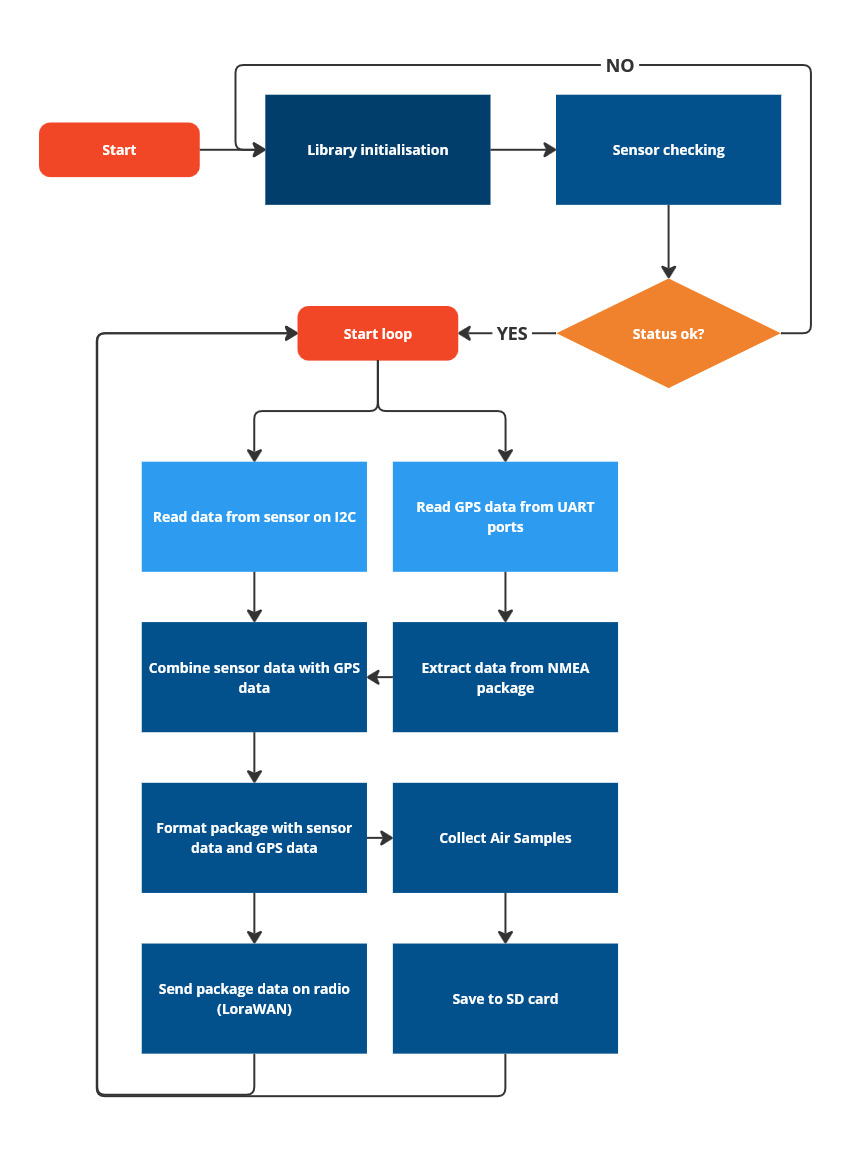
\includegraphics[width=9cm]{images/pdr/software diagram.jpg}
    \caption{\small{Software diagram.}}
    \label{fig:codeblocks}
\end{figure}

We will be using Git extensively to keep track of changes to the codebase. This allows us to easily roll back to a previous version if a new feature breaks the code. With Git, we can collaborate on the codebase and track changes made by different team members, ensuring a smooth and efficient development process.

% \begin{wrapfigure}{r}{0.5\textwidth}
%     \centering
%     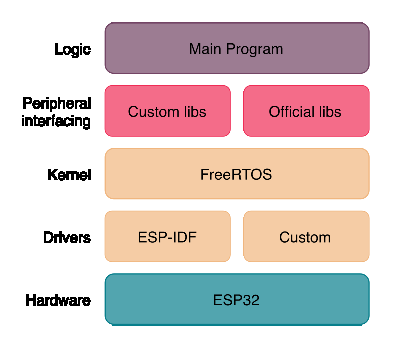
\includegraphics[width=7.5cm]{images/img_Cansat_RTOS.eps}
%     \caption{\small{CanSat software state diagram.}}
%     \label{fig:rtos}
% \end{wrapfigure}


Additionally, we are planning to develop a custom software application that will run on the ground station. This application will receive the telemetry data from the payload and interpret it, visualizing the information on real-time graphs. The software will extract sensor data such as acceleration, GPS coordinates, pressure, and more from the raw data packets, allowing us to monitor the payload's performance and the environmental conditions it encounters. The software will also log the data to ensure that no valuable measurements are lost. 